\section{Prototype}
For this thesis a tool was developed that easily allows to cluster companies by different feature weights,
select the most appropriate cluster from all the cluster combinations emerged by a hierarchical clustering
and visualize this cluster and show the important information and statistics for each group.

\begin{figure}[ht]
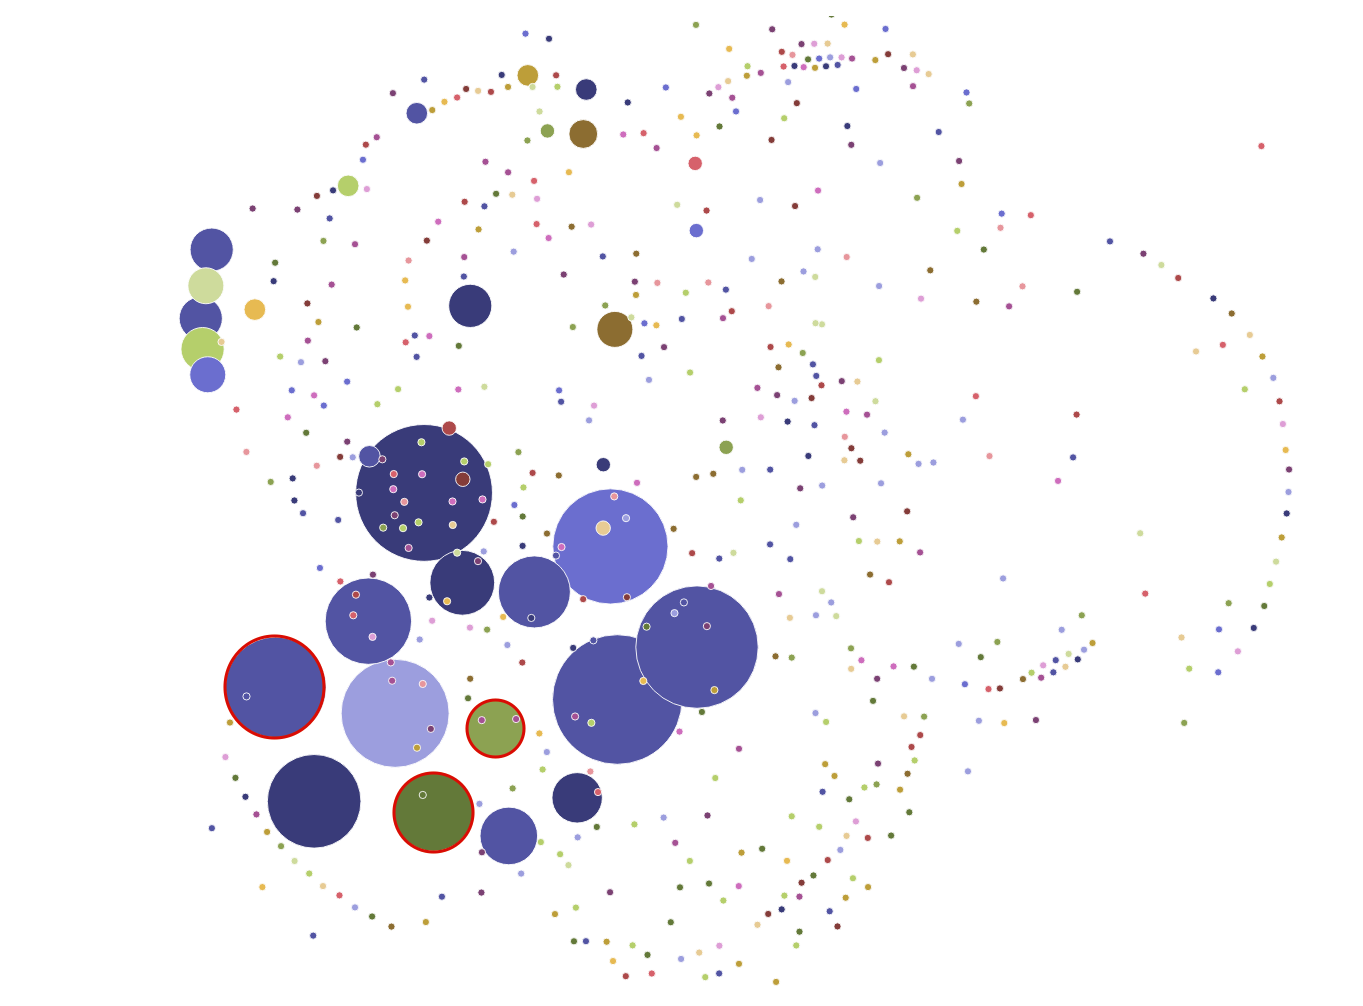
\includegraphics[width=0.6\linewidth]{clusterVisualization.png}
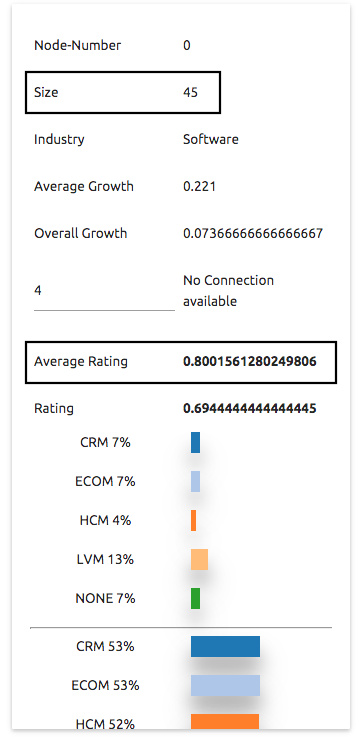
\includegraphics[width=0.3\linewidth]{clusterStats.png}
\centering
\caption{A cluster visualization}
\label{fig:clusterVisualization}
\end{figure}

Figure \ref{fig:clusterVisualization} shows an example visualization of clusters produced by the tool.
Each circle represents an own cluster. The bigger each circle's radius, the more companies are contained within this cluster.
The distance between each cluster shows their distance towards each other. Circles with a red border include companies
that raised a demand in a timeframe that can be adjusted. The different coloring of the clusters illustrates the dominant industry.
A click on a cluster gives an overview of the most important
values, as what needs were raised, what is the clusters or the overall demand distribution for all products or what is
the accordingly cluster score.
